\section*{Anexos}
\addcontentsline{toc}{section}{Anexos}

\begin{figure}[H]
	\centering
	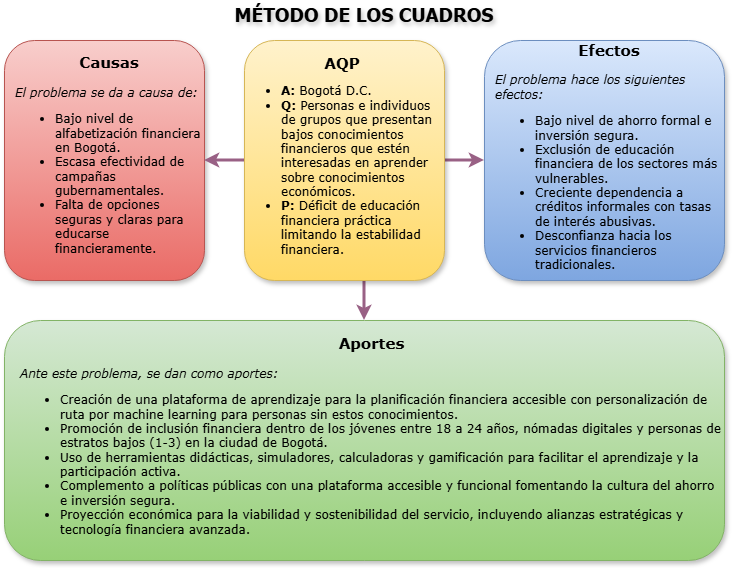
\includegraphics[width=12cm]{Imagenes/MetodoCuadros.png}
	\caption[{Método de los cuadros.}]{\centering Método de los Cuadros. \textit{Fuente:} Autores.}
	\label{fig:metodocuadros}
\end{figure}

\begin{adjustbox}{
		center,
		caption=[{Matriz de problemas y objetivos.}]{\centering Matriz de problemas y objetivos. \textit{Fuente:} Autores.},
		label={MatrizProblemasObjetivos},
		nofloat=table, vspace={20px}}
	\resizebox{\textwidth}{!}{
		\begin{tabular}{|c|c|}
			\hline
			\rowcolor[HTML]{F5B8B8}
			\multicolumn{2}{|c|}{\begin{tabular}[c]{@{}c@{}} \textbf{Matriz de problemas y objetivos}\end{tabular}} \\ \hline
			\rowcolor[HTML]{FAD4D4} 
			\textbf{Problemas} & \textbf{Objetivos} \\ \hline
			\rowcolor[HTML]{F7E9E9} 
			\textit{Problema General} & \textit{Objetivo General} \\ \hline
			\begin{tabular}[c]{@{}c@{}}¿Cómo puede una plataforma digital de asesoramiento \\ financiero superar las barreras asociadas a la baja alfabetización \\ financiera y la limitada personalización de contenidos, \\ para brindar orientación accesible, confiable y adaptada \\ a las necesidades de diversos perfiles de usuarios, promoviendo una \\ mejora real en sus hábitos económicos y maximizando el impacto social \\ y la sostenibilidad del modelo de negocio? \end{tabular} &
			\begin{tabular}[c]{@{}c@{}}Diseñar un plan de negocios para un servicio digital de \\ planificación financiera, didáctico y personalizado mediante \\ tecnologías y uso de machine learning dirigido a personas jóvenes, \\ informales y otros que estén interesadas en aprender sobre educación \\ financiera, que incluye herramientas interactivas para mejorar \\ la compresión de temas económicos y facilitar la toma de decisiones \\ responsables sobre presupuesto, interés, entre otros. \end{tabular} \\ \hline
			\rowcolor[HTML]{F7E9E9} 
			\textit{Problemas Específicos} & \textit{Objetivos Específicos} \\ \hline
			\begin{tabular}[c]{@{}c@{}}¿Cómo superar la baja alfabetización financiera que \\ limita a las personas a tomar decisiones económicas \\ informadas?\end{tabular} & \begin{tabular}[c]{@{}c@{}} Incrementar la alfabetización mediante uso de herramientas educativas \\ claras, simuladores y asesoría adaptadas a sus necesidades \end{tabular} \\ \hline
			\begin{tabular}[c]{@{}c@{}}¿Cómo diseñar un servicio accesible y adaptado que \\ incluya asesoría y herramientas digitales para ayudar a la \\ gestión  financiera personal?\end{tabular} & \begin{tabular}[c]{@{}c@{}} Desarrollar una plataforma digital amigable la cual tenga asesoramiento \\ financiero  personalizado apoyado por machine learning para mejorar \\ el manejo de presupuesto, ahorro y deudas. \end{tabular} \\ \hline
			\begin{tabular}[c]{@{}c@{}}¿Cómo disminuir la exclusión financiera de grupos vulnerables \\ como jóvenes, trabajadores independientes e informales y \\ personas en  la economía de Bogotá\end{tabular} & \begin{tabular}[c]{@{}c@{}} Facilitar la inclusión financiera de grupos vulnerables al \\ ofrecer un servicio que atienda a sus particularidades superando \\ barreras tecnológicas y sociales. \end{tabular} \\ \hline
		\end{tabular}
	}
\end{adjustbox}